% !TeX program = xelatex
% !BiB program = xelatex

\documentclass[landscape,twocolumn,a5paper]{manual}
\usepackage[margin=0.33in,bottom=0.5in,footskip=0.25in]{geometry}

\usepackage{tikz}
\usetikzlibrary{positioning,shapes,backgrounds}
\usepackage{tkz-euclide}
\usepackage{cleveref}

\definecolor{themered}{HTML}{284b81}
\colorlet{theme}{themered}

\renewcommand{\arraystretch}{1.5}

\definecolor{highlightcolour}{HTML}{DEE6EF}
\newcommand\shortcut[1]{\colorbox{highlightcolour}{\texttt{#1}}}

\pluginname{ChowMatrix}

\def\pluginfolder{\href{https://help.uaudio.com/hc/en-us/articles/210216306-Default-Install-Locations-for-UAD-Plug-Ins}{plugin folder}}
\def\dllink#1{\href{https://github.com/jatinchowdhury18/AnalogTapeModel/releases}{#1}}

\begin{document}

\section{ChowMatrix User Manual}

\noindent
\boldtheme{ChowMatrix} is an infintely growable delay
matrixing effect. The fundamental idea of the effect is
to create a ``tree'' of delay lines, each with it's own
proprties, such as delay-time, feedback, paning, etc.
This flexibility allows musicians and producers to create
a wide array of delay-based effects, from simple multi-tap
echoes, to lush reverberant spaces.The plugin is currently
available as VST/VST3/AU/LV2 for Windows, Linux, and Mac.

\subsection{Installation}
To install ChowMatrix for Mac or Windows, download the
\dllink{latest release}, unzip the downloaded file, and copy
the plugin files to your \pluginfolder. Note that Macintosh
users may need to
\href{https://www.imore.com/how-open-apps-anywhere-macos-catalina-and-mojave}{allow applications from unidentified developers}.
Linux users may 
\href{https://github.com/Chowdhury-DSP/ChowMatrix#Building}{compile from source}.

\begin{figure}[ht]
    \center
    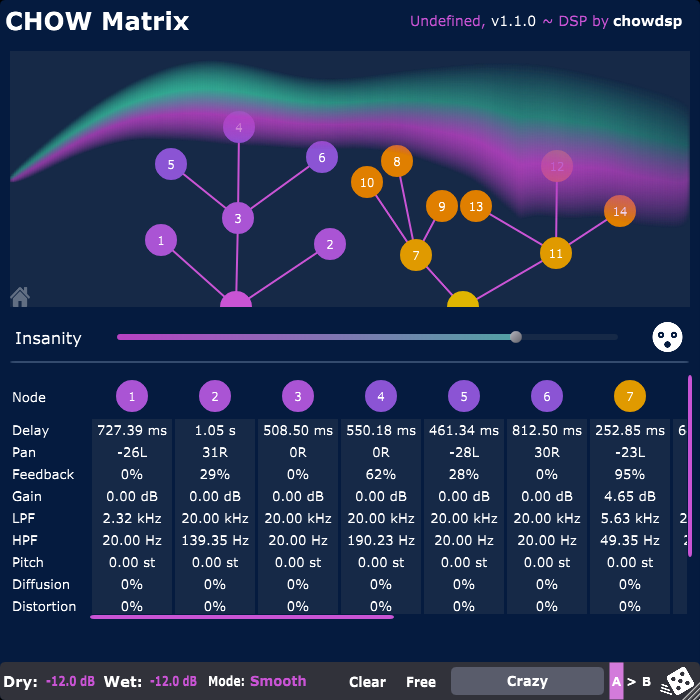
\includegraphics[width=0.75\columnwidth]{screenshots/full_gui.png}
    \caption{\label{fig:full_gui}{\it ChowMatrix User Interface}}
\end{figure}

\subsection{Processing}
The way in which ChowMatrix processes audio may not
be immediately obvious, especially compared with more
``traditionally'' designed audio plugins. ChowMatrix is
made up a ``tree'' of delay ``nodes'', where each node has
a ``parent'' node and potentially one or more ``child'' nodes.
The tree has two ``root'' nodes, representing the left and right
input channels to the plugin. Each node accepts a mono input
from its parent node, passes a mono signal on to its children,
and outputs a stereo signal to the main plugin output.

\subsubsection{Delay Nodes}
Each delay node consists of a delay line, as well as a gain,
highpass filter, lowpass filter, diffusion filter, distortion,
pitch-shifter, a global feedback path, and panner. The full
processing architecture for a single delay node is shown in
\cref{fig:delay_dsp}.
\newpar
%
\begin{figure*}
    \centering
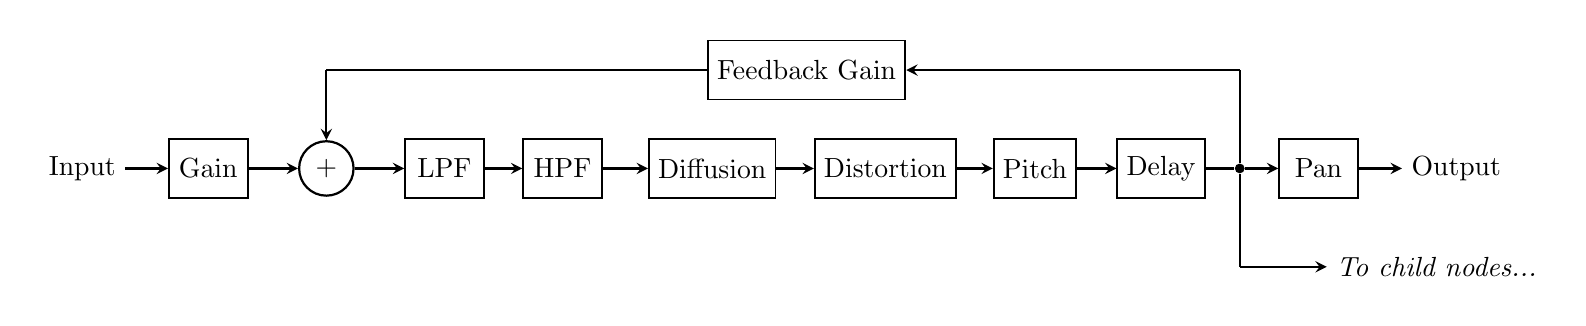
\begin{tikzpicture}[node distance=1.5cm, background rectangle/.style={fill=white}, show background rectangle]
    \tikzset{
        mynode/.style = {rectangle, line width=0.65pt, minimum width=1.0cm, minimum height=0.75cm, text centered, draw=black, fill=white},
        amp/.style = {regular polygon, regular polygon sides=3, draw, fill=white, text width=1em,
                      inner sep=1mm, outer sep=0mm, shape border rotate=-90, line width=0.8pt},
        arrow/.style = {thick,->,>=stealth},
    }
    \node (input) {Input};
    \node (gain) [mynode, right of=input, xshift=0.1cm] {Gain};
    \node (sum) [draw, fill=white, circle, line width=0.8pt, right of=gain] {+};
    \node (lpf) [mynode, right of=sum] {LPF};
    \node (hpf) [mynode, right of=lpf] {HPF};
    \node (diff) [mynode, right of=hpf, xshift=0.4cm] {Diffusion};
    \node (dist) [mynode, right of=diff, xshift=0.7cm] {Distortion};
    \node (pitch) [mynode, right of=dist, xshift=0.4cm] {Pitch};
    \node (delay) [mynode, right of=pitch, xshift=0.1cm] {Delay};
    \node (split) [circle, fill, inner sep=1.25pt, right of=delay, xshift=-0.5cm] {};
    \node (pan) [mynode, right of=split, xshift=-0.5cm] {Pan};
    \node (output) [right of=pan, xshift=0.25cm] {Output};

    \draw [arrow] (input) -- (gain);
    \draw [arrow] (gain) -- (sum);
    \draw [arrow] (sum) -- (lpf);
    \draw [arrow] (lpf) -- (hpf);
    \draw [arrow] (hpf) -- (diff);
    \draw [arrow] (diff) -- (dist);
    \draw [arrow] (dist) -- (pitch);
    \draw [arrow] (pitch) -- (delay);
    \draw [thick] (delay) -- (split);
    \draw [arrow] (split) -- (pan);
    \draw [arrow] (pan) -- (output);

    \coordinate[above of=split, yshift=-0.25cm] (up);
    \node (fb) [mynode, left of=up, xshift=-4cm] {Feedback Gain};
    \coordinate[above of=sum, yshift=-0.25cm] (over);
    \draw [thick] (split) -- (up);
    \draw [arrow] (up) -- (fb);
    \draw [thick] (fb) -- (over);
    \draw [arrow] (over) -- (sum);

    \coordinate[below of=split, yshift=0.25cm] (down);
    \node (children) [right of=down, xshift=1.0cm] {\it To child nodes...};
    \draw [thick] (split) -- (down);
    \draw [arrow] (down) -- (children);
\end{tikzpicture}
    \caption{\label{fig:delay_dsp}{\it Signal flow for a single delay node.}}
\end{figure*}
%
The input \boldtheme{Gain} applies a simple gain
to the signal before being processed by the delay
node. Adjusting the gain can be useful for making
certain delay nodes louder/quieter in the mix.
\newpar
The \boldtheme{Lowpass/Highpass} filters are simple
first-order filters with adjustable cutoff frequencies.
Note that since the filters are in the feedback loop,
the filtering process will be applied recursively to every
``echo'' of the signal through the feedback loop.
\newpar
The \boldtheme{Diffusion} filter is a multi-stage allpass
filter, that ``smears'' out the signal across the delay line.
Using diffusion in combination with feedback for rhythmic
and percussive sounds, can create an interesting effect.
\newpar
\boldtheme{Distortion} applies an anti-aliased waveshaping
distortion\footnote{Anti-aliasing is done without oversampling using anti-derivative anti-aliasing. For more information, see: \href{http://dafx16.vutbr.cz/dafxpapers/20-DAFx-16_paper_41-PN.pdf}{Parker et. al., 2016}.}
to the the signal. As with the filters, note that this
distortion will be applied recursively to the echos created
by the feedback path.
\newpar
The \boldtheme{Pitch} processor re-pitches the signal up
or down by a given number of semitones. This effect can be
useful for obtaining interesting and creative soundscapes.
\newline
The \boldtheme{Delay} line has a length that can be
controlled either as a ``free'' parameter, with units
of milliseconds, or synced to the tempo of the song.
\newpar
The \boldtheme{Feedback} gain controls how much of the
delayed signal is fed back to the input.
Setting the feedback to control to its maximum value
enables \boldtheme{Freeze} mode, which freezes the
current signal in the delay line, and mutes any incoming
input signal.
\newpar
The \boldtheme{Pan} processor applies a constant-power
panner to the mono signal processed by the delay node,
turning it into a stereo signal that is then fed to the
plugin output.

\subsubsection{Modulation}
Each delay node also contains modulations controls for the
delay time and panning. The modulation section has three
controls:
\newpar
\boldtheme{Mod Freq} determines the modulation frequency.
Similar to the delay length, the modulation frequency can
be controlled as either a free parameter (0 - 5 Hz), or
synced to the tempo of the song.
\newpar
\boldtheme{Delay Mod} controls the amount the delay length
is modulated for this node. Note that changing the
\hyperlink{goto:interp-mode}{delay interpolation mode}
will change how this modulation sounds.
\newpar
\boldtheme{Pan Mod} controls the modulation amount for
the node pan control. Note that this control can be
set to negative values to reverse the modulation.

\subsection{Controls}
The ChowMatrix interface is made up of four main sections:
the ``Graph View'', ``Details View'', ``Bottom Bar''
and ``Insanity Control''.

\begin{figure}[ht]
    \center
    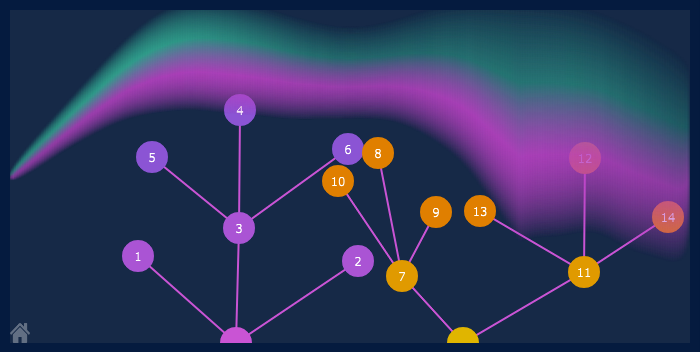
\includegraphics[width=0.8\columnwidth]{screenshots/GraphView.png}
    \caption{\label{fig:graph_view}{\it ChowMatrix Graph View}}
\end{figure}

\subsubsection{Graph View}
The \boldtheme{Graph View} is the main interface for interacting
with the delay nodes and managing the connections between nodes,
as well as providing an informative and inspiring visualization
of the delay processing being performed by the plugin.
\newpar
At the bottom of the graph view are two \boldtheme{Input Nodes},
represented by half-circles. The Input Node on the left represents
the left input channel, and the right Input Node represents the right
input channel.
\newpar
To \boldtheme{create} a new
node, \shortcut{SHIFT+Click} on the background of the Graph
View. If a node is selected, the new node will be created
as a ``child`` of the selected node. If no node is selected,
the new node will be created as a child of the nearest Input
Node.
\newpar
To \boldtheme{select} a node, simply click on the node. A menu
will appear showing the parameter controls for the selected node.
To un-select, simply click the background of the Graph View.
\newpar
When you \shortcut{Click+Drag} to \boldtheme{move} a node,
the panning and delay time of that node will change accordingly.
The panning is controlled by the node's angle relative to its
``parent'' node, and the delay line is controlled by the distance
from the node to its parent.
\newpar
To \boldtheme{delete} a node,
\shortcut{CMD+Click} on the node, or press the \shortcut{Delete}
key when the node is selected.
\newpar
To \boldtheme{solo} the audio from a specific node,
\shortcut{ALT+Click} on the node. To un-solo the node,
click on the background of the Graph View.
\newpar
The mouse can be used to explore the far reaches of the
Graph View by scrolling, or clicking and dragging. Click
the \boldtheme{Home} icon in the bottom left corner, to
return to the default view position.

\begin{figure}[ht]
    \center
    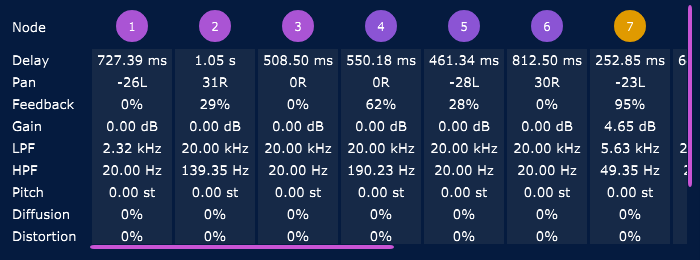
\includegraphics[width=0.9\columnwidth]{screenshots/DetailsView.png}
    \caption{\label{fig:details_view}{\it ChowMatrix Details View}}
\end{figure}

\subsubsection{Details View}
The \boldtheme{Details View} is below the Insanity Slider
on the interface, and allows the user to view and edit the
parameters for each node without having to select the node
in the Graph View.
\newpar
To select a node in the Details View, click the corresponding
node circle. Note that selecting a node in the Details
View will select the same node in the Graph View.
\newpar
To edit a parameter, \shortcut{Click+Drag} on the parameter
value. Alteratively, single-clicking on the value allows
you to type in a value for the parameter. Double-clicking
will reset the parameter to its default value.
\newline
Using \shortcut{SHIFT+Click+Drag}
will change the same parameter for all the delay nodes in
unison. \shortcut{CMD+Click} on a value to ``lock'' the
parameter so that it will not be affected by the ``Insanity''
control.

\subsubsection{Insanity Control}
ChowMatrix also features an \boldtheme{Insanity} parameter.
By turning up the Insanity, the plugin will allow the delay
nodes to ``wander'' randomly, with a speed and intensity
determined by the parameter value. Insanity is useful for
finding new delay node configurations, or for adding a source
of chaotic modulation.

\begin{figure}[ht]
    \center
    
\includegraphics[width=0.95\columnwidth]{screenshots/BottomBar.png}
    \caption{\label{fig:details_view}{\it ChowMatrix Bottom Bar}}
\end{figure}

\subsubsection{Bottom Bar}
The ``Bottom Bar'' section includes several auxiliary controls,
as well as a presets menu.
\newpar
The \boldtheme{Dry/Wet} sliders control the level of the dry
and wet signals coming out of the plugin. To use ChowMatrix as
a ``send'', turn the Dry level all the way down to \texttt{-inf}.
\newpar
\hypertarget{goto:interp-mode}{\boldtheme{Mode}} controls
the delay interpolation mode\footnote{For more information on
delay-line interpolation, see \href{https://ccrma.stanford.edu/~jos/pasp/Delay_Line_Signal_Interpolation.html}{Smith III, 2010}.}
used by the delay nodes. Using higher-order interpolation modes
will make the delay nodes sound more ``smooth'' when the delay
length is changed, at the cost of slightly higher CPU usage.
First-order interpolation will make the delay nodes sound ``rough''
when the delay length is changed, as well as attenuating high
frequencies passing through the delay. Zero-order interpolation
will make the delay nodes sound  ``glitchy'' when the delay length
is changed. The differences between the delay modes are most noticeable
when moving the delay nodes quickly, particularly in ``Insane'' mode,
and are further accentuated when lots of feedback is used.
\newpar
\boldtheme{Clear} will flush all signal from the delay nodes.
This can be useful if you have delay nodes with lots of feedback,
and wish to clear the delay lines without having to wait for
the feedback to echo until silence.
\newpar
\boldtheme{Sync/Free} toggles whether the delay times are synced
to the tempo of the song, or ``free'' to be any length.
\newpar
The \boldtheme{A/B} control allows the user to toggle
between two plugin states. This can be useful for using
insanity mode without losing your current settings. Use
the ``A'' or ``B'' buttons to load one of the saved states
as the current active state. Use the ``arrow'' button to
save the current state as either the A or B state.
\newpar
The \boldtheme{Randomise} button will randomise the parameters
for all the delay nodes. This can be useful for quickly
dicovering new delay node configurations.

\subsection{Presets}
Presets provide a quick way to achieve a specific sound
with the plugin. ChowMatrix comes with a set of built-in
factory presets. To contribute your presets to be added
to the factory presets list for future releases, please
email me.

\subsubsection{User Presets}
To save the current plugin state as a user preset, open
the presets menu, and select ``Save''. The first time a
preset is saved, you will be asked to choose a preset
folder. All future presets will be saved to this folder,
and when the plugin opens, it will search this folder, as
well as any subfolders, to load new user presets.
Presets located in subfolders will be placed in their
own groups in the preset menu.

\subsection{Open Source}
ChowMatrix is open-source software that is free (as in ``free
beer''), and free (as in ``free speech''), under the
3-clause BSD license.
\newpar
As an open-source project, ChowMatrix is
open to outside contributors. If you would like to contribute
to the development of ChowMatrix, please visit the
\href{https://github.com/Chowdhury-DSP/ChowMatrix/issues}{issues page}
for a list of outstanding tasks. If you would like to implement
a new feature, please create an issue ticket first, so the
feature can be discussed by the community.

\subsection{Feedback}
If you notice any bugs, or have any questions, feel free
to \href{mailto:chowdsp@gmail.com}{email me directly},
or \href{https://github.com/Chowdhury-DSP/ChowMatrix/issues}{create an issue ticket}
on GitHub. GitHub issues are preferred, since they are publicly
visible.
\newpar
Enjoy!
\newpar
Jatin Chowdhury
\newpar
\href{https://github.com/Chowdhury-DSP/ChowMatrix}{https://github.com/Chowdhury-DSP/ChowMatrix}

\newpage
\subsection{Shortcuts}
\begin{center}
    \begin{tabular}{| c || c | c |} 
    \hline
    \boldtheme{Action} & \boldtheme{Shortcut} & \boldtheme{Item} \\
    \hline
    Add Node & \texttt{SHIFT+Click} & Graph View \\
    Delete Node & \texttt{CMD+Click} & Graph View \\
    Solo Node & \texttt{ALT+Click} & Graph View \\
    \hline
    Unison Change & \texttt{SHIFT+Drag} & Param Slider \\
    Insanity Lock & \texttt{CMD+Click} & Param Slider \\
    Set to default & \texttt{Double-Click} & Param Slider \\
    Freeze Mode & $>95\%$ & Feedback Slider \\
    Tempo-sync LFO & \texttt{CMD+Click} & Mod. Freq. Slider \\
    \hline
   \end{tabular}
\end{center}

\end{document}
